Curve fitting is a very common theme in pattern recognition. The concept of invariant functions convey mapping functions that approximate a discriminating function when a parent function is reduced from a high dimensional space to a low dimensional space \cite{mallat2016understanding}.  In this chapter an invariance function called a scattering transform  enables invariance of groups of deformations that could apply to speech signals thereby preserving higher level characterisations useful for classifying speech sounds. Works done by \citep{peddinti2014deep,zeghidour2016deep,anden2011multiscale,sainath2014deep} have shown that when the scattering spectrum are applied to speech signals and used as input to speech systems have state of the art performance.  In particular \cite{sainath2014deep} shows 4-7\% relative improvement in word error rates (WER) over Mel frequencies cepstral coefficients (MFCCs) for 50 and 430 hours of English Broadcast News speech corpus.  While experiments have been performed with hybrid HMM-DNN systems in the past, this thesis focuses on the use of scatter transforms in end-to-end RNN speech models.

This chapter iterates the use of the Fourier transform as the starting analysis function for building invariant functions and then discusses the Mel filter bank solution and then establishes why the scattering transform through the wavelet modulus operator provides better invariance features over the Mel filters.

\section{Fourier transform}
The Fourier transform often referred to as the power spectrum, allows us to discover frequencies contained within a function.  The Fourier transform is a convolution between a signal and a complex sinusoid from $-\infty$ to $+\infty$ (Figure \ref{fig_4_1_fourier_eqn}). 

\begin{figure}
\centering
  % Requires \usepackage{graphicx}
  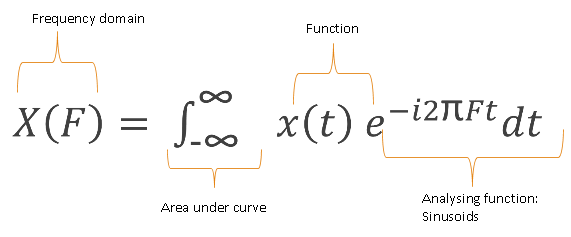
\includegraphics[width=7cm]{thesis/images/fourier.png}\\
  \caption{Fourier Equation} \label{fig_4_1_fourier_eqn}
\end{figure}
From the orthogonal property of complex exponential function, two functions are orthogonal if $\int f(x)g(x)=0$ where f(x) and g(x) are complimentary functions, one being referred to as the analysis equation and the other referred to as the synthesis function.

If the discrete form of the Fourier transform analysis equation is given by
\begin{equation}
a_k=\frac{1}{T}\int_{-T/2}^{T/2}x(t)e^{\left(-j\frac{2\pi kt}{T}\right)}
\label{eqn_c4_fourier01}
\end{equation}

Then, the corresponding synthesis equation is given by
\begin{equation}
x(t)=\sum_{k=-\infty}^{\infty}a_ke^{\left(j\frac{2\pi kt}{T}\right)}
\label{eqn_c4_fourier02}
\end{equation}

Recall that $x(t)$ is the original signal while $a_k$ is the Fourier Series coefficient.  This coefficient indicates the amplitude and phase of the original signal's higher order harmonics indexed by $k$ such that higher values of $k$ correspond to higher frequency components.  In a typical spectrogram (figure \ref{fig_4_2_spectral}), it can be seen that the energy of the signal is concentrated about a central region and then harmonic spikes of energy content exponentially decrease and taper off.  Therefore in figure \ref{fig_4_2_spectral}, the energies are concentrated at frequencies of about 100, 150 and 400 hertz.
\begin{figure}
\centering
  % Requires \usepackage{graphicx}
  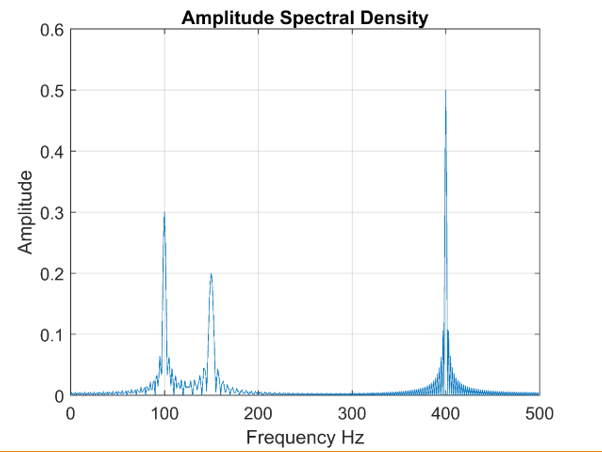
\includegraphics[width=7cm]{thesis/images/spectral.png}\\
  \caption{Sample Spectrogram} \cite{xxx}\label{fig_4_2_spectral}
\end{figure}

The Fourier transform discussed in the previous section constitutes a valuable tool for the analysis of the frequency component of a signal.  However is not able to determine when in time a frequency occurs hence is not able to analyse time related signal deformations.  The Short-time Fourier Transform (STFT) attempts to salvage this by windowing the signal in time signal and performing Fourier transforms over sliding windows sections of the original signal rather than the whole signal.  There is however, a resolution trade off that ensues from this operation such that, the higher the resolution in time accuracy, the lower the frequency accuracy and vice versa.  In the next section on the continuous wavelet transform, how the wavelet transform improves on the weaknesses of the Fourier Transform and the STFT is reviewed.

\section{Wavelet transform}
The continuous wavelet transform can be defined as a signal multiplied by scaled and shifted version of a wavelet function $\psi(t)$ referred to as the mother wavelet. The time-frequency tile-allocation of the three basic transforms examined in the first part of this chapter is illustrated in figure \ref{fig_4_3_tftile}

\begin{figure}
\centering
  % Requires \usepackage{graphicx}
  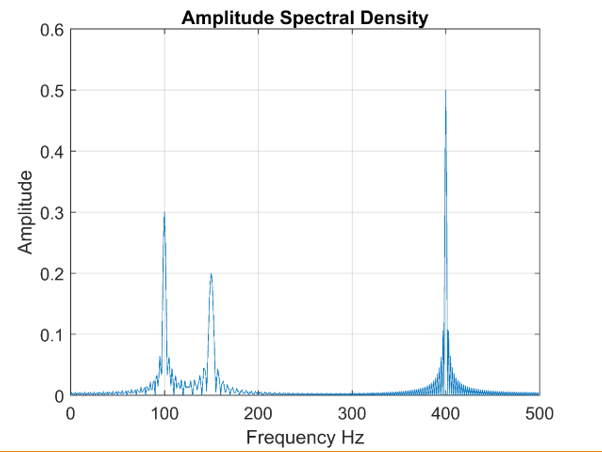
\includegraphics[width=7cm]{thesis/images/spectral}\\
  \caption{Time frequency tiling for (a) Fourier Transform (b) Short-time Fourier Transform (STFT) (c) Wavelet transform}\label{fig_4_2_tftile}
\end{figure}

It can be seen here that for the Fourier transform there is no time information obtained.  In the STFT, as there is no way of telling where in time the frequencies are contained, the STFT makes a blanket range of the resolution of the window and is therefore equally tiled potentially losing information based on this setup.  For the case of the wavelet, because it is a scaled and shifted convolution, it takes care of the this problem providing a good resolution in both time and frequency.  The fundamental representation of the continuous wavelet function is:
\begin{equation}
C(a,b)=\int f(t)\frac{1}{\sqrt{a}}\psi\left(\frac{t-b}{a}\right)dt\label{eqn_c4_wavelet01}
\end{equation}
In this equation, $a$ and $b$ respectively represent the scaling and shifting resolution variables of the wavelet function. This is referred to as a mother wavelet. A few other mother wavelet functions discussed later in this chapter. Generally a mother wavelet is identified as being energy spikes in an infinite signal whose accumulative energy sums to zero.

\section{Discrete and Fast wavelet transform}
Synthesis and analysis equations (\ref{eqn_c4_fourier02} and \ref{eqn_c4_fourier01}) can be formulated as a linear combination of the basis $\phi_k(t)$ such that the basis, $\phi_k(t)=e^{j2\pi kt}$, and it's conjugate or orthonormal basis, $\tilde{\phi}_k(t)=e^{-j2\pi kt}$, equations (\ref{eqn_c4_fourier02} and \ref{eqn_c4_fourier01}) now become

\begin{equation}
x(t)=\sum_{k}a_k\phi_k
\label{eqn_c4_dwt02}
\end{equation}

\begin{equation}
a_k=\int x(t)\tilde{\phi}_k(t)
\label{eqn_c4_dwt01}
\end{equation}

With respect to scaling and shifting variables of continuous wavelet transforms in equation (\ref{eqn_c4_wavelet01}), a similar linear combination transformation can be applied by constructing orthonormal bases parameters, referred to as scaling ($\phi$) and translating ($\psi$) functions. For example, a simple Haar mother wavelet transform associated with a delta function, it is seen that:
\begin{equation}
\phi_{j,k}(t)=2^{j/2}\phi(2^jt-k)
\label{eqn_c4_dwt03}
\end{equation}
\begin{equation}
\psi_{j,k}(t)=2^{j/2}\psi(2^jt-k)
\label{eqn_c4_dwt04}
\end{equation}
where j is associated with the dilation (scaling) parameter and k is associated with the position (shifting) parameter. If the Haar coefficients $h_{(\cdot)}[n]=\{1/\sqrt{2},1/\sqrt{2}\}$ are extracted we have the following dilation and position parameters.
\begin{equation}
\phi(t)=h_\phi[n]\sqrt{2}\phi(2t-n)
\label{eqn_c4_dwt05}
\end{equation}
\begin{equation}
\psi(t)=h_\phi[n]\sqrt{2}\psi(2t-n)
\label{eqn_c4_dwt06}
\end{equation}

For any signal, a discrete wavelet transform in $l^2(\mathbb{Z})^1$ can be approximated by
\begin{equation}
f[n]=\frac{1}{\sqrt{M}}\sum_kW_\phi[j_0,k]\phi_{j_0,k}[n]+\frac{1}{\sqrt{M}}\sum_{j=j_0}^\infty\sum_kW_\psi[j,k]\psi_{j,k}[n]
\label{eqn_c4_dwt07}
\end{equation}
Here $f[n],\phi_{j_0,k}[n]$ and $\psi_{j,k}[n]$ are discrete functions defined in [0,M - 1], totally M points.  Because the sets $\{\phi_{j_0,k}[n]\}_{k\in\mathbf{Z}}$ and $\{\psi_{(j,k)\in\mathbf{Z}^2,j\ge j_0}\}$ are orthogonal to each other.  We can simply take the inner product to obtain the wavelet coefficients.
\begin{equation}
W_\phi[j_0,k]=\frac{1}{\sqrt{M}}\sum_nf[n]\phi_{j_0,k}[n]
\label{eqn_c4_dwt08}
\end{equation}
\begin{equation}
W_\psi[j,k]=\frac{1}{\sqrt{M}}\sum_nf[n]\psi_{j,k}[n] \quad j\ge j_0
\label{eqn_c4_dwt09}
\end{equation}
Equation (\ref{eqn_c4_dwt08}) is called approximation coefficient while (\ref{eqn_c4_dwt09}) is called detailed coefficients.

These two components show that the approximation coefficient, $W_\psi[j_0,k]$, models a low pass filter and the detailed coefficient,$W_\psi[j_0,k]$, models a high pass filter. It is possible to determine the approximation and detailed coefficients without the scaling and dilating parameters. The resulting coefficients, called the fast wavelet transform, are a convolution between the wavelet coefficients and a down-sampled version of the next order coefficients.  The fast wavelet transform was first postulated in \citep{mallat1989theory}.

$$W_\phi[j,k]=h_\phi[-n]\ast W_\phi[j+1,n]|_{n=2k, k\ge 0}$$
\label{eqn_c4_dwt10}
\end{equation}
\begin{equation}
$$W_\psi[j_0,k]=h_\psi[-n]\ast W_\phi[j+1,n]|_{n=2k, k\ge 0}$$
\label{eqn_c4_dwt11}
\end{equation}

For analysis of the Haar wavelet and the derivation of equations (\ref{eqn_c4_dwt10} and \ref{eqn_c4_dwt11}) see appendix \ref{app01}.

## Mel filter banks

Mel Frequency Cepstral Coefficents (MFCCs) are a feature widely used in automatic speech and speaker recognition. They were introduced by Davis and Mermelstein in the 1980's, and have been state-of-the-art ever since. Prior to the introduction of MFCCs, Linear Prediction Coefficients (LPCs) and Linear Prediction Cepstral Coefficients (LPCCs) and were the main feature type for automatic speech recognition (ASR), especially with HMM classifiers. 

An audio signal is constantly changing, so to simplify things we assume that on short time scales the audio signal doesn't change much (when we say it doesn't change, we mean statistically i.e. statistically stationary, obviously the samples are constantly changing on even short time scales). This is why we frame the signal into 20-40ms frames. If the frame is much shorter we don't have enough samples to get a reliable spectral estimate, if it is longer the signal changes too much throughout the frame.

The next step is to calculate the power spectrum of each frame. This is motivated by the human cochlea (an organ in the ear) which vibrates at different spots depending on the frequency of the incoming sounds. Depending on the location in the cochlea that vibrates (which wobbles small hairs), different nerves fire informing the brain that certain frequencies are present. Our periodogram estimate performs a similar job for us, identifying which frequencies are present in the frame.

The periodogram spectral estimate still contains a lot of information not required for Automatic Speech Recognition (ASR). In particular the cochlea can not discern the difference between two closely spaced frequencies. This effect becomes more pronounced as the frequencies increase. For this reason we take clumps of periodogram bins and sum them up to get an idea of how much energy exists in various frequency regions. This is performed by our Mel filterbank: the first filter is very narrow and gives an indication of how much energy exists near 0 Hertz. As the frequencies get higher our filters get wider as we become less concerned about variations. We are only interested in roughly how much energy occurs at each spot. The Mel scale tells us exactly how to space our filterbanks and how wide to make them. 

Once we have the filterbank energies, we take the logarithm of them. This is also motivated by human hearing: we don't hear loudness on a linear scale. Generally to double the percieved volume of a sound we need to put 8 times as much energy into it. This means that large variations in energy may not sound all that different if the sound is loud to begin with. This compression operation makes our features match more closely what humans actually hear. Why the logarithm and not a cube root? The logarithm allows us to use cepstral mean subtraction, which is a channel normalisation technique.

The final step is to compute the DCT of the log filterbank energies. There are 2 main reasons this is performed. Because our filterbanks are all overlapping, the filterbank energies are quite correlated with each other. The DCT decorrelates the energies which means diagonal covariance matrices can be used to model the features in e.g. a HMM classifier. But notice that only 12 of the 26 DCT coefficients are kept. This is because the higher DCT coefficients represent fast changes in the filterbank energies and it turns out that these fast changes actually degrade ASR performance, so we get a small improvement by dropping them.

## Deep scattering spectrum
In this section reference is made to \citep{anden2011multiscale, anden2014deep, zeghidour2016deep}. For a signal $$x$$ we define the following transform $$W_x$$ as a convolution with a low-pass filter $$\phi$$ and higher frequency complex analytic wavelets $$\psi_{\lambda_1}$$:
\begin{equation}
$$Wx=(x\star\phi(t),x\star\psi_{\lambda_1}(t))_{t\in\mathbb{R},\lambda_1\in\Lambda_1}$$ \label{eqn_c4_dss01}
\end{equation}

We apply a modulus operator to the wavelet coefficients to remove complex phase and extract envelopes at different resolutions
\begin{equation}
$$|W|x=\left(x\star\phi(t),|x\star\psi_{\lambda_1}(t)|\right)_{t\in\mathbb{R},\lambda_1\in\Lambda_1}$$ \label{eqn_c4_dss02}
\end{equation}
$$S_0x=x\star\phi(t)$$ is locally invariant to translation thanks to the time averaging $$\phi$$.  This time-averaging loses the high frequency information, which is retrieved in the wavelet modulus coefficients $$|x\star\psi_{\lambda_1}|$$.  However, these wavelet modulus coefficients are not invariant to translation, and as for $$S_0$$, a local translation invariance is obtained by a time averaging which defines the first layer of scattering coefficients
\begin{equation}
$$S_1x(t,\psi_{\lambda_1})=|x \star\psi_{\lambda_1}| \star\phi(t)$$\label{eqn_c4_dss03})
\end{equation}
It is shown in \cite{anden2014deep} that if the wavelets $$\psi_{\lambda_1}$$ have the same frequency resolution as the standard mel-filters, then the $$S_1x$$ coefficients approximate the mel-filter coefficients.  Unlike the mel-filter banks however, there is a strategy to recover the lost information, by passing the wavelet modulus coefficients  $$|x\star\phi_{\lambda_1}|$$ through a bank of higher frequency wavelets $$\psi_{\lambda_2}$$:
\begin{equation}
$$|W_2||x\star\phi_{\lambda_1}|=\left(|x\star\psi_{\lambda_1}|\star\phi,||x\star\psi_{\lambda_1}|\star\psi_{\lambda_2}|\right)_{\lambda_2\in\Lambda_2}$$ \label{eqn_c4_dss04})
\end{equation}
This second layer of wavelet modulus coefficients is still not invariant to translation, hence we average these coefficients with a low-pass filter $$\phi$$ to derive a second layer of of scattering coefficients.
 \begin{equation}
$$|W_2||x\star\phi_{\lambda_1}|=\left(|x\star\psi_{\lambda_1}|\star\phi,||x\star\psi_{\lambda_1}|\star\psi_{\lambda_2}|\right)_{\lambda_2\in\Lambda_2}$$ \label{eqn_c4_dss04})
\end{equation}

Repeating these successive steps of computing invariant features and retrieving lost information leads to the scattering spectrum, as seen in Fig. 1, however speech signals are almost entirely characterized by the first two layers of the spectrum, that is why a two layers spectrum is typically used for speech representation. It is shown in [6] that this representation is invariant to translations and stable to deformations, while keeping more information than the mel-filter banks coefficients

![alt text](https://raw.githubusercontent.com/deeperj/dillinger/master/thesis/images/scatter.png "Scattering network - 2 layers deep")
\begin{figure}
\centering
  % Requires \usepackage{graphicx}
  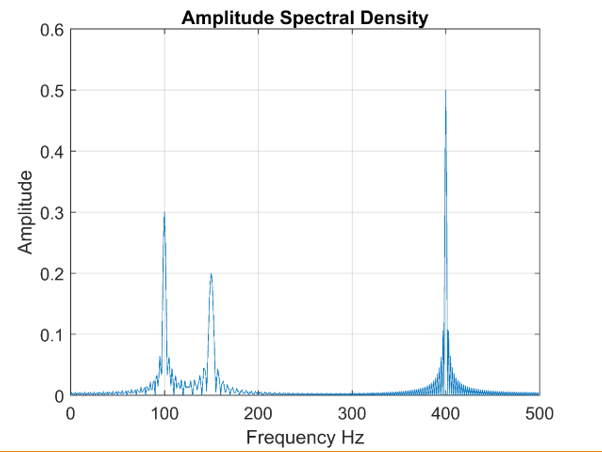
\includegraphics[width=7cm]{thesis/images/spectral.png}\\
  \caption{Scattering network - 2 layers deep} \cite{zeghidour2016deep}}\label{fig_4_3_scatter}
\end{figure}
